% !TEX root = thesis.tex
\chapter{Preliminaries}

\section{Combinatorial Models}

Our basic objects of study will be graphs and simplicial complexes.
In general,
by
a combinatorial model for a group $G$,
we mean any graph or simplicial complex
whose automorphism group is naturally isomorphic to $G$.



\subsection{Graphs and Simplicial Complexes}

In the discussion below a \emph{graph}
will be a collection of vertices equipped with a collection of edges that are unordered pairs of vertices.
We will allow graphs to have
multiple, parallel copies of edges between
a given pair of vertices, which we call multi-edges,
as well as edges $vv$ for a single vertex $v$, which we call self-loops.
We call any graph \emph{simple} if it has no multi-edges or self-loops.
The \emph{simplification} of any graph is the simple graph obtained by removing any self-loops and identifying the parallel copies of each multi-edge into a single edge.
We say two vertices $v$ and $w$ are \emph{adjacent} if $vw$ is an edge, and we say two edges are
\emph{incident} if they share a vertex, or else say an edge is incident to its two vertices.

We will typically consider  a \emph{simplicial complex}
$\mathcal C$ purely combinatorially as a set of vertices $\mathcal C^{(0)}$ equipped with a set of simplices,
so an $n$-simplex is a set of $n+1$ vertices, and the faces of the simplex are the nonempty subsets.
The $n$-skeleton $\mathcal C^{(n)}$ of the complex $\mathcal C$ is the subcomplex of all $k$-simplices of $\mathcal C$ for $k \leq n$.
For any subset $V$ of vertices, the \emph{induced} subcomplex on $V$ contains a simplex of $\mathcal C$ if and only if it is a subset of $V$.
By the \emph{link} of a vertex $v$,
we mean the
induced subcomplex of the vertices adjacent to $v$.

Occasionally we will abuse notation by failing to differentiate between a simplicial complex and its geometric realization.
In particular, dimensions, interior points of simplices, and homotopy properties all refer to the geometric realization of a graph or a complex, rather than the combinatorial object itself.

Most of the simplicial complexes here considered are formed roughly like this:
\begin{enumerate}
  \item Choose a space $X$.
  \item Take as vertices of the complex all the homotopy classes of particular subspaces of $X$ of a particular topological type
  \item Declare a collection of homotopy classes to span a simplex if they have representatives that can be homotoped so that they are all mutually disjoint in $S$
\end{enumerate}
Such a simplicial complex is typically \emph{flag},
meaning that a set of vertices form a simplex if and only if they span a clique in the 1-skeleton $\mathcal C^{(1)}$. Since the one skeleton is a graph, we will frequently refer to the 1-simplices of a flag complex as edges.

Just as it is convenient to reduce higher simplices to their edges,
so too do actions on the edges frequently determine actions on vertices.
We recall Whitney's Graph Isomorphism Theorem
\cite{MR1506881}, which
states that the edge-incidence relation determines a simple graph,
with a single exceptional pair.

\begin{theorem}
  An edge-incidence preserving bijection between two simple, connected graphs
  is a isomorphism, provided neither is the complete graph $K_3$.

  There is an edge-incidence preserving edge bijection between the complete
  graph $K_3$ and the complete bipartite graph $K_{1,3}$.
  \label{thm:whitney}
\end{theorem}

\begin{figure}[h!]
  \centering
  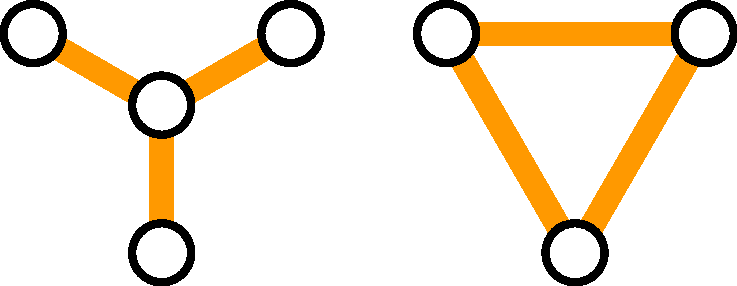
\includegraphics[width=.5\textwidth]{figures/graphexamples.pdf}
  \caption{
  The complete bipartite graph $K_{1,3}$ and the triangle $K_3$ are the only simple graphs
  are not isomorphic yet have an incidence preserve bijection of edges.
  }
  \label{fig:graphexamples}
\end{figure}

One classical consideration of graph theory
is the problem of chromatic numbers:
How many colors are required to
tag the vertices of a graph so that adjacent vertices have distinct colors?
We will require a slight generalization where each vertex instead requires a given number of colors and adjacent vertices must share no color.
One could replace vertices by cliques and consider classical colorings,
but this introduces additional automorphisms to a graph, so we will instead consider colorings by disjoint sets of specified size.

\begin{definition}
  A $k,\eta$-coloring of a graph $G=(V,E)$
  is an assignment
  to each vertex $v$ of a number of colors $\eta(v)$
  and
  a choice $f(v) \subset \{1,\ldots,k\}$ of $\eta(v)$
  colors
  such that two adjacent vertices have no common colors.
  I.e. a function $\eta: V \to \Z_+$ and  $f: V \to 2^{\{1,\ldots,k\}}$
  so that $|f(v)| = \eta(v)$
  and
  $$f(v) \cap f(u) = \varnothing$$
  if $v$ is adjacent to $u$ in $G$.
  Call $G$ $k,\eta$-colorable if it admits a $k,\eta$-coloring,
  and uniquely $k,\eta$-colorable if there is only one $k,\eta$-coloring up to bijection of the color set $k$.
  We will abusively refer to a $k,\eta$-coloring as a coloring if $k$ and $\eta$ are clear in context.
  \label{def:color}
\end{definition}

We will see in Chapter \ref{chap:birman} that complexes of based loops and spheres are uniquely colorable by the base points.


\subsection{Putman's Lemma}

In \cite{putman} Putman outlines a clever and versatile argument
for establishing the connectivity of a simplicial complex that admits a group action.
Putman points out that it suffices to show that
there is a special basepoint $v_0$ whose orbit intersects every connected component, and a special generating set $H$ such that $H\cdot v_0$ has paths to $v_0$.
This trick reduces many connectivity arguments to
a few trivial checks---if the generating set can be chosen so that most elements leave the base point $v_0$ fixed
or move it only a short distance.
We will make abundant use of the following Lemma.


\begin{lemma}
  \label{lemma:putman}
  Let group $G$ have generating set $H$ and act on simplicial set $X$.
  Fix a basepoint $v \in X^{(0)}$.
  If
  \begin{enumerate}
  \item for all $v' \in X^{(0)}$ the orbit $G\cdot v$ intersects the connected component of $v'$ in $X$ and
  \item for all $h \in H^{\pm}$ there is some path from $v$ to $h\cdot v$
  \end{enumerate}
  then $X$ is connected.
\end{lemma}

\begin{proof}
  By \emph{(1.)} it suffices to show that there is a path from $v$ to $g \cdot v$ for every $g \in G$.
  Writing $g$ as a word of $H$ we may factor $g= h_w \cdots h_1 \cdot v$ as a word of $\in H^{\pm}$.
  By hypothesis there is a path $s_j$ from  $ v$ to $ h_j \cdot v$
  Then
  $$
  s_1 \  (h_1h_2h_1^{-1} \cdot s_2)  \ldots (h_1 \cdots h_{k-1}) h_k (h_1 \cdots h_{k-1})^{-1} \cdot s_k
  $$
  is a path from $v$ to $g\cdot v$.
\end{proof}

We suggest a modification of Putman's Lemma that we will use to establish the uniqueness of the coloring of a complex.
Let $\Gamma$ be a graph with sets $V$ and $V'$ of vertices.
We say that a set $V$ \emph{forces} a coloring on $V'$ if for every $k,\eta$-coloring
$f$ of the induced subgraph of $\gamma$ with vertices $V$,
the extension of $f$ to $\gamma$ restricts to the same coloring on $V'$.

\begin{lemma}
  \label{putmancolor}
  Let group $G$ with generating set $H$ act on a graph $X$.
  Fix a collection $V \subset X^{(0)}$ of $k$ vertices.
  If
  \begin{enumerate}
  \item for every vertex $v \in X$ the orbit $G \cdot V$ forces a coloring on $v$, and
  \item for all $h \in H^{\pm}$ we have $V$ forces a coloring on $h\cdot V$
  \end{enumerate}
  then $V$ forces a coloring on $X$,
  and in particular $X$ is uniquely $k,\eta$-colorable.
\end{lemma}

\begin{proof}
  Observe that forcing a coloring is a transitive relation on subsets of vertices.
  It suffices to see that $V$ forces a coloring on its orbit $G\cdot V$, since the orbit forces a coloring on $X$.
  Suppose that $W$ and $W'$ are vertex sets such that $W$ forces a coloring on $W'$.
  Let $g \in G$.
  Then $g \cdot W$ must force a coloring on $g \cdot W$, or else we would have colorings
  $f$ of $W$ and two distinct colorings $f'$ and $f''$ of $W$ such that $f$ extends to colorings restricting to $f'$ and $f''$, and these pullpack to colorings $f \circ g$ of $W$, and $f'\circ g$, $f''\circ g$ of $W'$ contradicting that $W$ forces a coloring on $W'$.
  Then if $g= h_w \cdots h_1$ as a word of $\in H^{\pm}$
  we have $h_j \cdots h_1 \cdot V$ forces a coloring on $h_{j+1} \cdots h_1 \cdot V$,
  so that $V$ forces a coloring on $g \cdot V$ by transitivity.
\end{proof}


\subsection{Bass-Serre Theory}

We refer the reader to Serre \cite{SerreJeanPierre2003T}
and  for a fuller treatment of the theory of groups acting on trees.
These trees provide an algebraic abstraction of covering spaces.
In essence, if $X$ is a space with subspace $Y$, by considering all lifts of $Y$ to the universal cover $\tilde X$ we can form a tree whose vertices are the components of $\tilde X$ cut along all lifts of $Y$ and equipped with an action by $\pi_1(X)$
as the deck transformations of the cover $\tilde X$.


A \emph{graph of groups} $\Gamma$
is a connected graph $(V,E)$ together with
a collection of vertex groups $\{G_v\}_{v \in V}$
and a collection of edge groups $\{G_e\}_{e \in E}$
together with inclusions of the edge groups into their incident vertex groups, that is for each edge $e=uv$ there are injections
$$
\begin{tikzcd}
G_u & G_e \arrow[l,hook',"i_{uv}"] \arrow[r,hook,"i_{vu}"] & G_v.
\end{tikzcd}
$$

Then for any spanning tree $T$ of $\Gamma$
the fundamental group $\pi_1(\Gamma,T)$
is the group generated by $\{x_e\}_{e\in E}$ and the vertex groups $G_v$ for $v \in V$,
together with the relations
$i_{uv}(g) = x_e i_{vu}(g) x_e^{-1}$ for all $e=uv$
and $g \in G_e$,
and $x_e=1$ for all $e \in T$.

The universal cover $\tilde \Gamma$ of the graph of groups $\Gamma$ (with respect to $\pi_1(\Gamma, T)$) is the tree
with vertices
given by the left cosets of vertex groups in $\pi_1(\Gamma, T)$.
The edges are given by the left cosets of edge groups in $\pi_1(\Gamma, T)$.
So if $gG_e$ is the left coset of edge group $G_e$ with $g \in \pi_1(\Gamma, T)$
and edge $e=uv$, then
$gG_e$ is an edge
between the $\tilde \Gamma$ vertices $gG_u$ and $gx_eG_v$.
The quotient $p: \tilde \Gamma \to \Gamma$
is given by $gG_x \mapsto x$ for any vertex or edge.
In fact $\tilde \Gamma$ is a tree,
and is
equipped with
action
of $\pi_1(\Gamma, T)$ by left multiplication
$$
h \cdot \left ( gG_x \right) = (hg) G_x
$$
for any $g,h \in \pi_1(\Gamma, T)$.
The action of $\pi_1(\Gamma, T)$ on the tree
$\tilde \Gamma$ thus has
$$
\mbox{stab}_{\pi_1(\Gamma, T)} \left ( gG_x \right )
=
gG_xg^{-1}
$$
and respects the projection $p$ and acts without inverting any edges of the tree.
This tree action is unique in the sense described by the Fundamental Theorem of Bass-Serre Theory:

\begin{theorem}
  Let $T$ be a tree with group $G$ acting without inversions. If $\Gamma$ is the quotient graph of groups with $T$ any spanning tree,
  then $G$ is isomorphic to $\pi(\Gamma, T)$,
  and there is an $G$-equivariant isomorphism betweeen $T$ and the universal cover $\tilde \Gamma$ of $\Gamma$.
  \label{thm:bassserre}
\end{theorem}

\section{Surface Models}

We refer the reader to Farb and Margalit \cite{primer} as the definitive
treatment of surface topology and surface group algebra,
and to Hatcher \cite{MR1867354} for theory and notation of homotopy,
but we here establish notation and recall
some relevant results.

Let $S_{g,p}$ be the orientable genus $g$ surface with a set finite set $P$
of $p$ punctures.
The mapping class group is
$$\mcg(S_{g,p}) = \pi_0 \mbox{Diff}^+(S_{g,p})$$
the group of isotopy classes of orientation preserving homeomorpisms of $S_{g,p}$.
We will also consider the extended mapping class group of orientation reversing homeomorphisms
$$\mcg^{\pm}(S_{g,p}) = \pi_0 \mbox{Diff}(S_{g,p}).$$
By a \emph{curve} of $S_{g,p}$
we mean the homotopy class of a simple closed curve, an embedded copy of the circle $S^1$.
We will frequently abuse notation
by refering to a curve both as the embedding $S^1 \hookrightarrow S_{g,p}$
and its homotopy class, as dictated by context.
The same will be true of \emph{loops} which we consider to be pointed embeddings $(S^1,s_0) \hookrightarrow (S_{g,p},q)$ considered up to homotopy of $S_{g,p}$ fixing the basepoint $q$,
and \emph{arcs} which we consider to be
embedded intervals $([0,1],0,1) \hookrightarrow (S_{g,p},q_0,q_1)$
considered up to homotopy of $S_{g,p}$ fixing the endpoints $q_0$ and $q_1$ which we often allow to be punctures.
We will often refer to what Farb and Margalit call the \emph{change of coordinates principle}:
curves $x$ and $y$ lie in the same $\mcg$ orbit if
and only if their complements in $S_{g,p}$ are homeomorphic.
Thus the topological types of curves are
\emph{nonsepararing}, and \emph{separating} curves whose regular neighborhood complement is $S_{g'p'} \sqcup S_{g'',p''}$
where
$g=g'+g''$ and $p+2=p'+p''$.
For a separating curve $x$
we refer to the connected components of its complement as the \emph{sides}
of $x$, and the \emph{small side} as whichever has a less negative Euler characteristic.

\subsection{The Curve Complex}

Harvey defined the complex of curves $\mathcal C S_{g,p}$ as follows \cite{MR624817}.
Take as vertices all homotopy classes of simple closed curves.
A collection of curves forms a simplex if and only if
they are mutually disjoint.
Farb and Margalit give an extensive treatment in \cite{primer}.

The works of
Ivanov \cite{MR1460387},
Korkmaz \cite{MR1696431},
and
Luo \cite{MR1722024},
describe the automorphisms of complexes of curves.
Their theorem states that (except in a few low complexity cases)
the curve complex is a combinatorial model for the mapping class group.

\begin{restatable}{theorem}{curvecomplex}
  The natural map
  $$
  \mcg^\pm S_{g,p} \to  \aaut \mathcal C S_{g,p}
  $$
  is surjective whenever the curve complex
  $\mathcal C S_{g,p}$
  has positive dimension $3g+p-4$ and $(g,p) \neq (1,2)$,
  and an isomorphism if
  $(g,p) \notin \{(1,2),(2,0)\}.$
  \label{thm:curvecomplex}
\end{restatable}


\subsection{The Birman Exact Sequence}
The Birman exact sequence
describes the
mapping class group of a punctured surface
as a fibration
over the mapping class group of the unpunctured surface,
where the fundamental group is the fiber.
Given a specified point $q \in S_{g,p}$ and loop $\alpha: ([0,1],0,1) \to (S_{g,p},q,q)$ based at $q$
we can construct a \emph{point pushing map} that pushes
$q$ along the loop $\alpha$.
Construct the push map by taking an isotopy $H: [0,1] \times S_{g,p} \to S_{g,p}$
that is the identity outside of a neighborhood of $\alpha$ and so that $H(t,q) =\alpha(t)$ for all $t \in [0,1]$.
Then $H(0,\cdot)$ and $H(1,\cdot)$ are isotopic homeomophisms of $S_{g,p}$ relative to $P$, but are not isotopic relative $P\cup\{q\}$.
This embeds the fundamental group in the mapping class group as a subgroup of point-pushing maps in the group $\mcg^{\pm}(S_{g,p+1},q)$
of mapping classes fixing the point $q$.
The relationship is fully described by the following exact sequence
due to Birman \cite{MR0243519}.

\begin{restatable}{theorem}{birman}
    \label{thm:birman}
  Let $q\in S_{g,p}$ be a puncture for negative Euler-characteristic $S_{g,p}$.
  The surface inclusion
  $S_{g,p+1}=S_{g,p}-\{q\} \hookrightarrow S_{g,p}$
  induces the following short exact sequence
  $$
  1 \to
  \pi_1(S_{g,p},q) \to
  \mcg^{\pm}(S_{g,p+1},q) \to
  \mcg^{\pm}S_{g,p} \to
  1.
  % \begin{tikzcd}
  % 1 \arrow[r]&1
  % \pi_1(S_{g,p},q) \arrow[r]&
  % \mcg^{\pm}(S_{g,p+1},q)  \arrow[r]&
  % \mcg^{\pm}S_{g,p} \arrow[r]&
  % 1
  % \end{tikzcd}
  $$
\end{restatable}

Surprisingly, while the fundamental group of the surface is
normal in the mapping class,
we will see in the next section that the extended mapping class group itself is never normal in any supergroup,
except as a direct product.


\subsection{Mapping class group are only trivial normal subgroups.}

In general, a fibration of groups is an exact sequence
$$
\begin{tikzcd}
  1 \arrow[r] &
  A \arrow[r]&
  E \arrow[r]&
  B \arrow[r]&
  1
\end{tikzcd}
$$
and these are classified up to isomorphism
by the outer automorphisms $\oout A$ of the fiber $A$
and the cohomology $H^\ast (B;Z(A))$ of the base $B$.
We refer to Brown for a general theory \cite{MR1324339}.
But mapping class groups are centerless and out-less.
We prove here centerless and out-less fibers always make for trivial fibrations,
so fibrations with $\mcg$ as the fiber are always trivial
for sufficiently complex surfaces.
See Farb and Margalit \cite{primer} for centers of mapping class groups.

\begin{theorem}
  The center of $\mcg^{\pm} S_{g,p}$ is trivial, unless
  $$(g,p) \in \left\{ (0,2), (1,0),(1,1),(1,2),(2,0) \right\}$$
  and in all these cases the center is isomorphic to $\Z/2$.
  \label{nocenter}
\end{theorem}

The curve complex $\mathcal CS_{g,p}$
plays a large role in the proof that $\aaut \mcg^{\pm}S_{g,p} \cong \mcg^{\pm}S_{g,p}$.
The work of McCarthy \cite{MR830038}, Ivanov \cite{MR1460387}, Korkmaz \cite{MR1696431}
demonstrates the following theorem
showing that
$\oout \mcg^{\pm}S_{g,p} = 1$.

\begin{theorem}
Let $(g,p)$ have $g\geq 2$ and $g+p \geq 3$,
or $g=1$ and $p\geq 3$, or $g=0$ and $p \geq 5$.
Let $G$ and $G'$ be finite index subgroups of $\mcg^\pm S_{g,p}$.
Then any isomorphism $G\to G'$ is induced by an inner automorphism of $\mcg^\pm S_{g,p}$.
\label{outmod}
\end{theorem}


\begin{theorem}
  A centerless, out-less group always fibers trivially.

  Suppose that
  $$
  \begin{tikzcd}
    1 \arrow[r] &
    A \arrow[hook,r]&
    E \arrow[two heads]{r}{\rho}&
    B \arrow[r]&
    1
  \end{tikzcd}
  $$
  is a short exact sequence of groups.
  If $A$ has trivial center and outer automorphism group,
  then $E \cong A \times B$.
  \label{centerout}
\end{theorem}

\begin{proof}
Let $B = \langle S | R \rangle$
be a presentation for $B$.
For each $s\in S$ choose $e_s \in E$
so that $\pi(e_s) =s$.
Note that $A = \ker \rho$ is normal in $E$.
So the conjugation
$x \mapsto e_s x e_s^{-1}$
restricts to an automorphism of $A$.
By hypothesis $\aaut A = \mbox{Inn } A$,
so there must be $a_s \in A$ such that
$e_sx e_s^{-1} =a_s x a_s^{-1}$ for all $x \in A$.
Since
$$
\rho (e_s) = \rho (e_sa^{-1}_s) = s
$$
we may replace $e_s$ with $e_sa^{-1}_s$
so that $e_sxe^{-1}_s = x$ for all $x \in A$.
So $\langle e_s \rangle_{s \in S}$ commutes with $A$ in $E$.
But then if $\prod_i s_i \in R$ is a relation of $B$,
we have $\prod_i e_{s_i}  \in A$ by the exact sequence,
so $\prod_i e_{s_i} \in Z(A)$ is in the center of $A$.
But by hypothesis the center is trivial $Z(A) \cong 1$, so $\prod_i e_{s_i}=1$ in $E$.
So $s \mapsto e_s$ extends to a homomorphism $B \to E$ that splits the exact sequence,
and whose image commutes with $A$.
It must be that $E \cong A \times B$.
\end{proof}

\begin{corollary} The extended mapping class group has only trivial extensions.
  \label{cor:nomodextensions}
  Let $(g,p)$ have $g\geq 2$ and $g+p \geq 3$,
  or $g=1$ and $p\geq 3$, or $g=0$ and $p \geq 5$.
  Suppose that
  $$
  \begin{tikzcd}
    1 \arrow[r] &
    \mcg^{\pm} S_{g,p} \arrow[hook,r]&
    E \arrow[two heads]{r}&
    B \arrow[r]&
    1
  \end{tikzcd}
  $$
  is an exact sequence of groups.
  Then $E \cong B \times \mcg^{\pm} S_{g,p}$.
\end{corollary}

In particular the normalizer $N$ of $\mcg^{\pm} S_{g,p}$
in any group is a direct product  $\mcg^{\pm} S_{g,p} \times N/\mcg^{\pm} S_{g,p}$.


\section{Free Group Automorphism Models}

We write $F_n$ for the free group generated by $n$ elements.
The inner automorphisms given by conjugation are denoted $\mbox{Inn } F_n$
so that
$$
\oout F_n = \frac{\aaut F_n}{\mbox{Inn } F_n}
$$
We refer to Vogtmann for an excellent survery on
what is currently known about $\oout F_n$
\cite{VogtmannKaren2002Gd}, but here recall some
of the most relevant facts.

Let $a_1,\ldots,a_n$ be a generating set for $F_n$.
Elements of $\aaut F_n$
include
\begin{enumerate}
  \item a \emph{permutation} is an
  automorphism that permutes the generating set $\{a_1,\ldots,a_n\}$
  \item an \emph{inversion} at $a_i$ is an automorphism $\mu_i$
  extended from $\mu_i( a_i ) = a_i^{-1}$ and $\mu_i( a_j) = a_j$ for $j \neq i$.
  \item a \emph{transvection}
  is an automorphism $\tau_{ij}$ extended from
  $\tau_{ij}( a_i )= a_ia_j$ and $\tau_{ij}( a_k)= a_k$
  for $k \neq i$
\end{enumerate}
Nielson \cite{Nielsen1924} showed that $\aaut F_n$
can be generated by taking any basis $a_1,\ldots, a_n$ of $F_n$
and taking an inversion, a transposition,
and the permutations of $\{a_1,\ldots, a_n\}$.



Many results of
$\oout F_n$
are defined and proved analogously to
results on surface mapping class groups.
There are in fact several productive such analogies.
The first considers
elements of $\oout F_n$
as the mapping class group of graphs of rank $n$.
Since the graphs are one dimensional, to obtain $\oout F_n$ the
homotopy equivalences but be considered, rather than homeomorphism.
This is perhaps best explored by
Culler and Vogtmann \cite{MR830040},
who define  the \emph{outer space} of metrics on a graph
that functions for $\oout F_n$ just as Teichm\"uller space
does for surface mapping class groups.
Bridson-Vogtmann use techniques similar to Ivanov to show that
$\oout \oout F_n = \oout \aaut F_n=1$
\cite{MR1769698}.

A second analog instead considers $\oout F_n$
as the mapping class group of a doubled handlebody.
Let $M_{n}$ be the compact 3-manifold
that is the connect sum  $\#^n \left (S^1 \times S^2 \right )$.
Since $\pi_1(M_{n},x_0) = F_n$,
the diffeomorphisms of $M_n$ act on $F_n$ and provide a model for $\oout F_n$.
The 3-manifold $M_n$ makes an even closer analog to the surface $S_g$
since one way to construct $M_n$ is to take two copies of a genus $n$ handlebody and glue their boundary surfaces by the identity map.
To include boundary spheres, we let $M_{n,p}$ is the compact 3-manifold obtained
from $n$ copies of $S^1 \times S^2$ with
the interiors of $p$ disjoint balls removed.
We take the convention that $M_{0,p}$ is $S^3$ with the interiors of $p$ disjoint balls removed.
$\mbox{Diff}(M_{n,p})$ is the group of orientation-preserving diffeomorphisms of $M_{n,s}$.
Then the mapping class group of $M_n$
$\pi_0 \mbox{Diff}(M_{n,p}, \partial M_{n,p})$
can provide a model for $\oout F_n$.
The group $\pi_0 \mbox{Diff}(M_{n,p}, \partial M_{n,p})$
contains a finite normal subgroup $N$ generated by order 2 Dehn-twists about nonseparating spheres.
Laudenbach showed in \cite{MR0314054} that
$$
\frac{\pi_0 \mbox{Diff}(M_n)} N \cong \oout F_n
$$
and
$$
\frac{\pi_0 \mbox{Diff}(M_{n,1} ,\partial M_{n,1} )} N \cong \aaut F_n
$$
Since neither these groups nor the sphere complexes distinguish between removing a point or a ball from $M_n$,
we will abusively
also refer $M_n$ with a set $P$ of $p$ distinct points removed as $M_{n,p}$ where convenient,
and refer to the set $P$ as the punctures of $M_{n,p}$, since this sometimes unifies notation with the surface case.

For $p\geq 1$, discussion of \emph{relative} free groups or free groups with boundary can be found in Meucci \cite{MR2982242} and
Hatcher and Wahl \cite{MR2174267}.


Consider $F_{n+p}$ with basis $\{a_1,\ldots,a_n, b_1,\ldots, b_p\}$.
Let $\aaut_{n,p}$
be the subgroup $\aaut_{n,p}<F_{n+p}$
with $\phi \in \aaut_{n,p}$
if $\phi$ preserves the conjugacy class of $\langle a_1,\ldots, a_n \rangle$ and $\phi(b_i)$ is conjugate to $b_j$ for some $j$.
Let $\oout_{n,p} = \aaut_{n,p} / \mbox{Inn } F_{n+p}$.
An immediate consequence of the work of Hatcher and Vogtmann is
that $\pi_0 \mbox{Diff}(M_{n,p}) / N \cong \oout_{n,p}$
\cite{homstabout}.
In analogy with the pure mapping class group we will write
$$\pout_{n,p} \cong \pi_0 \mbox{Diff}(M_{n,p}, \partial M_{n,p}) / N$$
to be the subgroup $\pout_{n,p} < \oout_{n,p}$
that is the quotient from the subgroup of $\aaut _{n,p}$ with $\phi(b_i)$ conjugate to $b_i$ for all $i$.
So we have an exact sequence
$$
\begin{tikzcd}
1 \arrow[r] & \pout_{n,p} \arrow[r] & \oout_{n,p} \arrow[r] & \sym(p) \arrow[r] & 1
\end{tikzcd}
$$
where $\sym(p)$ is the symmetric group on $p$ symbols.
Similarly
let $\oout_{n,p}^{(q)}$
be the quotient of the $\aaut_{n,p}$ subgroup with $\phi(b_q)$ conjugate to $b_q$, so
$$
\begin{tikzcd}
1 \arrow[r] & \pout_{n,p} \arrow[r] & \oout^{(q)}_{n,p} \arrow[r] & \sym(p-1) \arrow[r] & 1
\end{tikzcd}
$$
Hatcher and Vogtmann provide a Birman type exact sequence for $M_n$.
Let $P$ be $p$ marked points in $M_n$ and $q \in M_n-P$.
There is a fibration
$$
\begin{tikzcd}
\mbox{Diff}(M_n,P\cup\{q\}) \arrow[r]&
\mbox{Diff}(M_n,P) \arrow[d]\\
&M_n-P
\end{tikzcd}
$$
where the projection is given by evaluation at $q$.
The  long exact sequence of homotopy groups
associated to the fibration yields a Birman-like short
exact sequence
$$
\begin{tikzcd}
  1 \arrow[r] &
  F_n \arrow[r] &
  \pi_0\mbox{Diff}(M_n,P\cup \{q\})) \arrow[r] &
  \pi_0\mbox{Diff}(M_n,P)) \arrow[r] &
  1
\end{tikzcd}
$$
which after a quotient by the finite normal Dehn-twist subgroup yields an exact sequence
$$
\begin{tikzcd}
  1 \arrow[r] &
  F_n \arrow[r] &
  \oout_{n,p+1}^{(q)} \arrow[r] &
  \oout_{n,p} \arrow[r] &
  1.
\end{tikzcd}
$$
So $\oout_{n,p}$ is generated by
\begin{enumerate}
  \item permutations of $\{a_1,\ldots,a_n\}$
  \item permutations of $\{b_1,\ldots,b_p\}$
  \item an $a$-inversion at $a_1$
  \item an $a$-transvection $\tau_{ij}$ with $\tau_{ij}(a_i)=a_ia_j$
  and $\tau_{ij}$ the identity on the other elements of the generating set
  \item a conjugation of $b_i$ by $a_j$ with $\gamma_{ij}(b_i)=a_jb_ia_j^{-1}$
  and $\gamma_{ij}$ the identity on the other elements of the generating set
\end{enumerate}


\begin{figure}[h!]
  \centering
  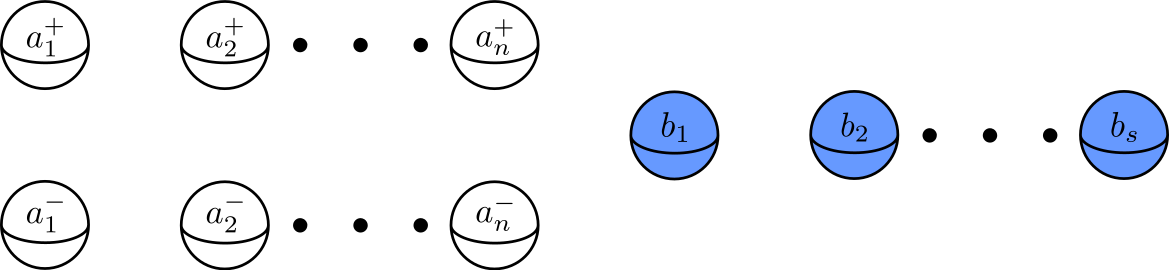
\includegraphics[width=\textwidth]{figures/spherestoglue.pdf}
  \caption{The manifold $M_{n,p}$ can be contained from  $S^3$
  by deleting the interior of $2n+p$ balls then identifying
  $n$ pairs of spheres via the antipodal map.}
  \label{fig:sphereglue}
\end{figure}


With this model of $\oout F_n$
the analog of the curve complex is the complex of embedded spheres in $M_n$.
Let $\mathcal S_{n,p}$
be the complex of spheres in $M_{n,p}$.
The vertices of $\mathcal S_{n,p}$ are
homotopy classes of essential, embedded 2-spheres $S^2 \hookrightarrow M_{n,s}$ in $\mathcal S_{n,p}$.
We will abuse notation and say \emph{sphere} to mean both a particular embedding $S^2\hookrightarrow M_{n,p}$
and its homotopy class, as dictated by context.
A set of spheres forms a simplex if there are mutually disjoint embeddings of the homotopy classes.
Hatcher showed that
the realization of $\mathcal S_{n}$
contains a dense subspace homeomorphic to Culler-Vogtmann outer space \cite{MR1314940}.
Aramayona and Souto showed that the sphere complex itself is
a combinatorial model for $\oout F_n$ \cite{souto}.

\begin{restatable}{theorem}{aramsouto}
\label{aramsouto}
The natural map $\oout F_n \to \aaut \mathcal S_n $ is an isomorphism for $n\geq 3$.
\end{restatable}

\begin{figure}[h!]
  \centering
  \includegraphics[width=.7\textwidth]{figures/samplecurves.pdf}
  \caption{
  A maximal collection of disjoint curves bounding disks in the handlebody.
  The prescribed doubling gives spheres of $M_3$
  specifying a maximal simplex of the sphere complex $\mathcal S_3$.
  }
  \label{fig:samplecurves}
\end{figure}

\begin{figure}[h!]
  \centering
  \includegraphics[width=.3\textwidth]{figures/samplespheres.pdf}
  \caption{
  A maximal collection of disjoint spheres of $S^3$ with spheres removed.
  The prescribed gluing gives spheres of $M_3$
  specifying a maximal simplex of the sphere complex $\mathcal S_n$.
  }
  \label{fig:samplespheres}
\end{figure}

There are two helpful diagramatic approaches to considering
spheres in $M_{n}$, shown in Figures \ref{fig:samplecurves} and \ref{fig:samplespheres}.
The first represents a sphere by  considering
a disk-bounding curve in a genus $n$ handlebody $H_n$,
$$x: (D^2,S^1) \hookrightarrow (H_n, S_n).$$
Then $x$ induces an embedding $x:S^2 \hookrightarrow M_n$
by taking two copies of $H_n$ and identifying the boundary
$\partial H_n = S_n$ of the two copies
$$
\begin{tikzcd}
  (D^2,S^1) \arrow[r] \arrow[d] &
  D^2 \sqcup_{S^1} D^2 \arrow[r] \arrow[d] &
  S^2 \arrow[d]  \\
  (H_n,S_n) \arrow[r]&
  H_n \sqcup_{S_n} H_n \arrow[r] &
  M_n.
\end{tikzcd}
$$
This gives a surjection from homotopy classes
of $(D^2,S^1)$ in $(H_n,S_n)$ to homotopy classes of $S^2$ in $M_n$,
but this representation by disks is not unique.
As in Figure \ref{fig:spheredisk}, Dehn twists about disk bounding curves intersecting $x$ give
distinct disks that glue up to give homotopic spheres in $M_n$.
The punctured manifold $M_{n,p}$ is similarly obtained by gluing a handlebody with $p$ half balls removed along the surface $S^p_n$.

\begin{figure}[h!]
  \centering
  \includegraphics[width=\textwidth]{figures/spheredisk.pdf}
  \caption{
   Identifying the two copies of a handlebody along their boundary obtains $M_n$ and glues disks into spheres. Disks differing by Dehn twists about curves bounding disks in the handlebody glue to the same sphere.
  }
  \label{fig:spheredisk}
\end{figure}

A second diagramatic representation is to consider cutting
$M_{n,p}$ along a collection of $n$ disjoint nonsepating spheres
to obtain $S^3$ with $2n+p$ open balls removed.
Label the resulting boundary $S^2$ spheres
$x^+_{a_1},\ldots,x^+_{a_n}$
and
$x^-_{a_1},\ldots,x^-_{a_n}$
and
$x_{b_1},\ldots,x_{b_p}$.
Then identifying $x^+_{a_i}$ and $x^-_{a_i}$ via the $S^2$ antipodal map obtains $M_{n,p}$ again.
Then for any basepoint $q \in M_{n,p}$
we have a basis for $F_n \cong \pi_1(M_{n,p},q)$
as $a_1, \ldots, a_n$
with $a_i$ the loop disjoint from $x_{a_j}$ for $j \neq i$
and intersecting $x_{a_i}$ once by traveling into
$x^+_{a_i}$
and out of
$x^-_{a_i}$, which we defined to be positive intersection.
Diffeomorphisms of $M_n,p$ realizing $\oout_{n,p}$
can be described using this model.
By capping every boundary component of
$M_{n,p}$ with a copy of $M_{1,1}$
we can include
 $\oout_{n,p} \hookrightarrow \oout F_{n+p}$
and consider diffeomorphisms of $M_{n+p,0}$
that preserve (setwise and with orientation) the set of separating spheres
where we glued the capping $M_{1,1}$ and the nonseparating spheres contained inside.

\begin{enumerate}
  \item Permutations $\sigma$ of $\{a_1,\ldots,a_n\}$ can be realized by any
  diffeomorphism sending sphere $x_{a_i}$ to $x_{\sigma(a_i)}$
  \item Inversion $\iota_1: a_1 \mapsto a_1^{-1}$
  can be realized by cutting $M_n$ along $x_{a_1}$
  exchanging the spheres $x^+_{a_1}$ and $x^-_{a_1}$
  and then regluing $x^+_{a_1}$ and $x^-_{a_1}$
  \item Transposition $\tau_{12}: a_1 \mapsto a_1a_2$
  can be realized by cutting $M_n$ along $x_{a_1}$,
  pushing $x^-_{a_1}$ along a loop that intersects $x_{a_2}$
  once negatively and disjoint from $x_{a_i}$ with $i\neq 1,2$,
  and finally regluing $x^+_{a_1}$ and $x^-_{a_1}$
  We will also refer to this as the push of $x^-_{a_1}$ through $x^-_{a_2}$.
  See Figure \ref{fig:transvect}.
  \item Conjugation $\eta: a_1 \mapsto a_1b_1a_1^{-1}$
  can be realized by  pushing $x_{b_1}$ along a loop that intersects $x_{a_1}$ once negatively and is disjoint from $x_{a_i}$ for $i \neq 1$
\end{enumerate}

\begin{figure}[h!]
  \centering
  \includegraphics[width=.6\textwidth]{figures/transvect.pdf}
  \caption{
  Pushing $x^-_{a_1}$ through $x^-_{a_2}$ induces the transvection $a_1 \mapsto a_1a_2$ on the fundamental group $\pi_1$.
  }
  \label{fig:transvect}
\end{figure}


By homotoping a sphere so that it is based at $q$,
we obtain a splitting of $\pi_1(M_n,q) \cong F_n$,
and in fact conjugancy classes of splittings of $F_n$ are in bijection with spheres of $M_n$.
By considering these splittings,
Handel and Mosher show that $\mathcal S_{n}$
is $\delta$-hyperbolic \cite{MR3073931}.



In \cite{MR1314940} Hatcher shows $\mathcal S_n$ is contractible and describes
a normal form for spheres embedded in $M_n$.
A maximal collection $\Sigma$ of disjoint spheres has $3n-3$ spheres. (One could, for example take the disks of a pants decomposition in the handlebody.)
Cutting $M_n$
along $\Sigma$ such a collection of spheres
produces $2n-2$ copies of $M_{0,3}$.
Hatcher shows that any sphere $x$ of $M_{n}$
can be homotoped so that $x$ is parallel to a sphere of
$\Sigma$ or meets them tranversely in a nonempty
colleciton of circles splitting $x$
into components $x_i$ such that
\begin{enumerate}
  \item Each component $x_i$ meets any sphere of $\Sigma$ in at most one circle.
  \item No component $x_i$ is a disk isotopic by an isotopy fixing its boundary to a disk in a sphere of $\Sigma$
\end{enumerate}
Further the homotopy class of $x$ is uniquely determined by the data of the components $x$ as a sphere parallel to a sphere of $\Sigma$, or else the components $x_i$ as a disk, annulus, or pair of pants in each component of $M_n$ cut along $\Sigma$, and the spheres of $\Sigma$ that $x_i$ boundary components intersect.

\begin{figure}[h!]
  \centering
  \includegraphics[width=.6\textwidth]{figures/normalform.pdf}
  \caption{
   The sphere for the splitting $\left \langle a_1^{-1}a_2^4 \right \rangle \ast \left \langle a_2,a_3 \right \rangle$ in Hatcher normal form with respect to the maximal collection $\{a_1,a_2,a_3,x,y,z\}$ in $M_3$.
  }
  \label{fig:normalform}
\end{figure}

Just as in the case of curves of the surface,
the spheres of a surface have a
{change of coordinates principle}:
spheres $x$ and $y$ lie in the same $\oout_{n,p}$ orbit if
and only if their complements in $M_{n,p}$ are homeomorphic.
Thus the topological types of spheres are
\emph{nonsepararing}, and \emph{separating} spheres whose complement is $M_{n'p'} \sqcup M_{n'',p''}$
where
$n=n'+n''$ and $p+2=p'+p''$.
For a separating sphere $x$
we refer to the connected components of its complement as the \emph{sides}
of $x$, and the \emph{small side} as whichever has a less negative Euler characteristic.
We refer to a sphere $y$ on the small side of $x$ as \emph{engulfed} by $x$,
or \emph{engulfed} if it lies on the large side of $x$.

Pandit has shown that the nonseparating spheres
also constitute a combinatorial model for $\oout F_n$ \cite{pandit}.
That is let $\nosep  \subset \mathcal S_n$ be the induced subcomplex spanned by nonseparating spheres. Pandit gives
\begin{theorem}
  For $n \geq 3$ the natural map
  $$\outn \to \Aut{\nosep}$$
  is an isomorphism.
\end{theorem}
